\documentclass[aspectratio=1610,handout]{beamer}

\usepackage[utf8]{inputenc}
\usepackage{polski}
\usetheme{ATH}
\usefonttheme{serif,professionalfonts}
\usepackage{graphicx}
\usepackage{caption}
\graphicspath{ {./img/} }

\theoremstyle{definition}
 \newtheorem*{def*}{Definicja}
 
\title{Aplikacja z graficznym interfejsem użytkownika do przetwarzania obrazów}
\author[Bartosz Dobija]{Bartosz Dobija}
\institute{Uniwersytet Bielsko-Bialski\\ Wydział Budowy Maszyn i Informatyki}

\date[5 lutego 2024]{Obrona pracy inżynierskiej \\ Bielsko-Biała, 5 lutego 2024}

\begin{document}

\begin{frame}{$ $}
    \titlepage
\end{frame}

\begin{frame}{Cel i zakres pracy}
    Celem tej pracy jest zaprojektowanie i implementacja oprogramowania do przetwarzania obrazów z funkcjonalnym interfejsem graficznym.
    \vspace{1cm}

    Aplikacja wymagała:
    \begin{itemize}
        \item analizy istniejących rozwiązań,
        \item wyboru technologii,
        \item zaimplementowanie metod przetwarzania obrazów,
        \item stworzenie interfejsu graficznego.
    \end{itemize}
\end{frame}

\begin{frame}{Projekt}
    Aplikacja NoodleCV pozwala na obsługę części biblioteki OpenCV za pomocą edytora węzłowego.

    \begin{figure}
            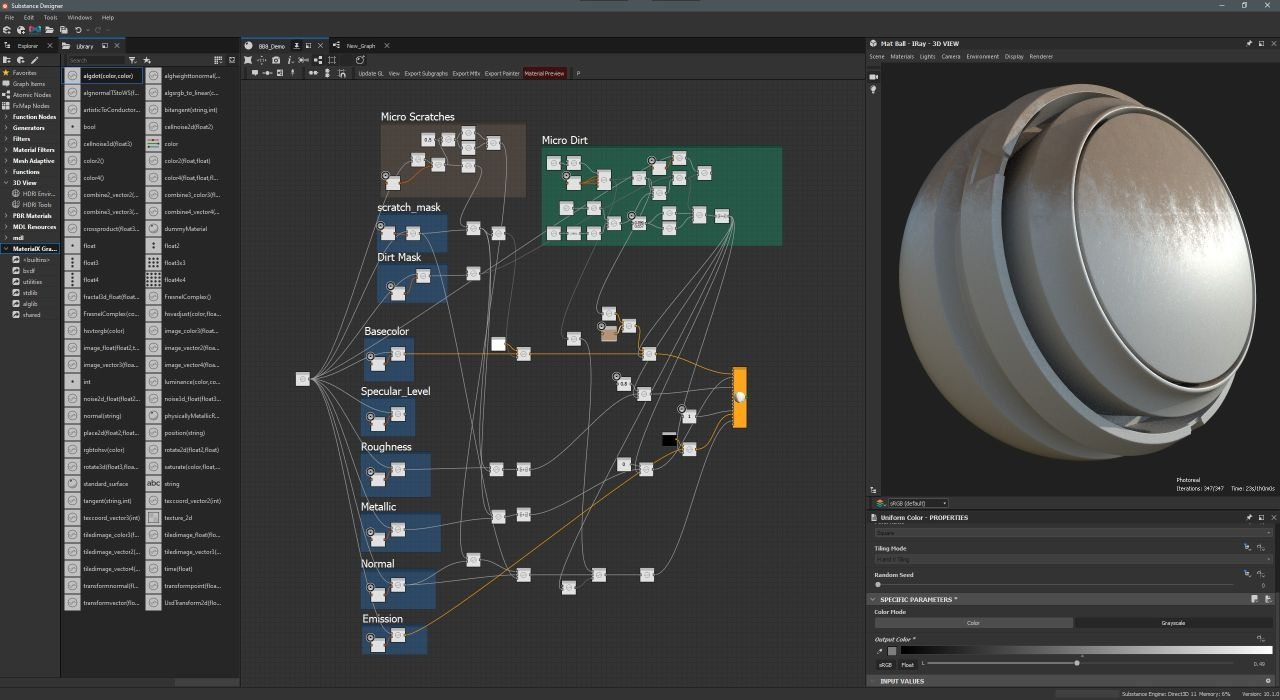
\includegraphics[height=3.9cm]{./imgs/substance.jpg}%
            \hfil
            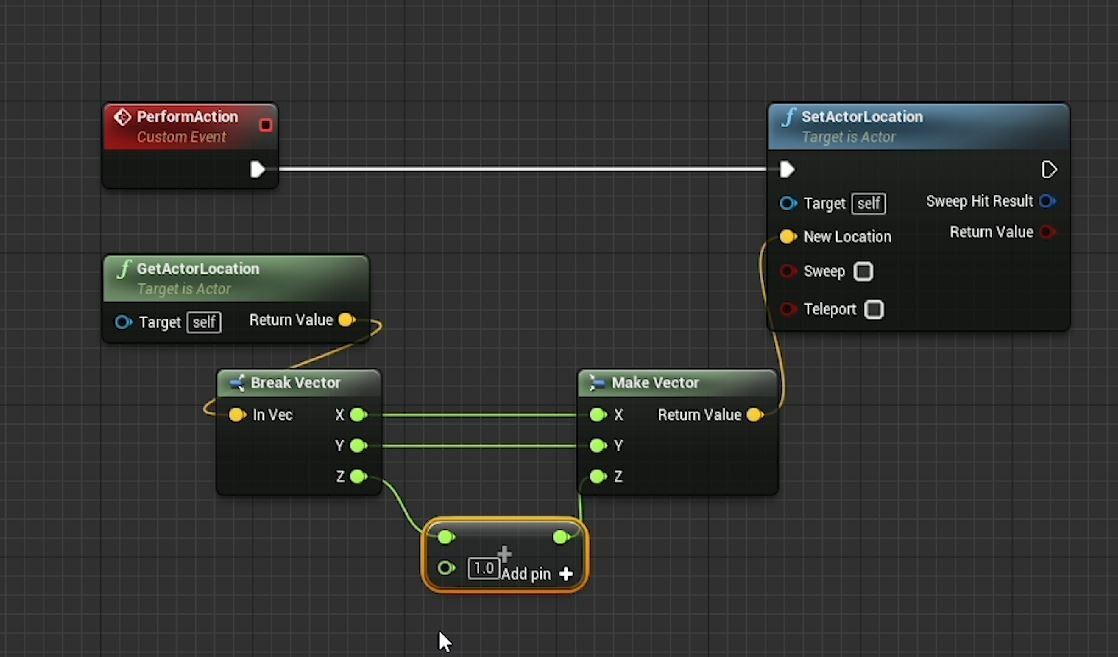
\includegraphics[height=3.9cm]{./imgs/unreal.JPG}
            \caption{Przykłady edytorów węzłowych.}
    \end{figure}

\end{frame}

\begin{frame}{Technologie i narzędzia}
 \begin{columns}[t]
        \column{.5\textwidth}
        \centering
        
\includegraphics[height=3cm]{./imgs/csharp.png}
        \captionof{figure}{Język programowania - C\#.}
        
\includegraphics[height=3cm]{./imgs/nodify.png}
        \captionof{figure}{Edytor węzłowy - Nodify.}
        \column{.5\textwidth}
        \centering
        
\includegraphics[height=3cm]{./imgs/wpfui.png}
        \captionof{figure}{Biblioteka komponentów - WPFUI.}
        
\includegraphics[height=3cm]{./imgs/OpenCV.png}
        \captionof{figure}{Przetwarzanie obrazów - OpenCV.}
    \end{columns}
\end{frame}

\begin{frame}{Architektura}
    \begin{figure}
            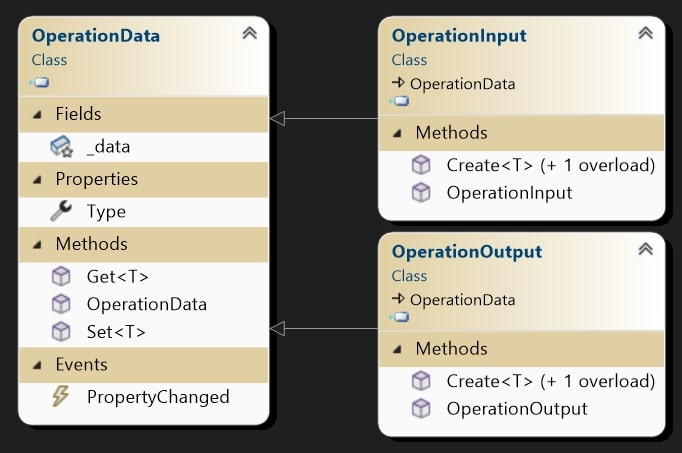
\includegraphics[height=5.3cm]{./imgs/generyczne.jpg}%
            \hfil
            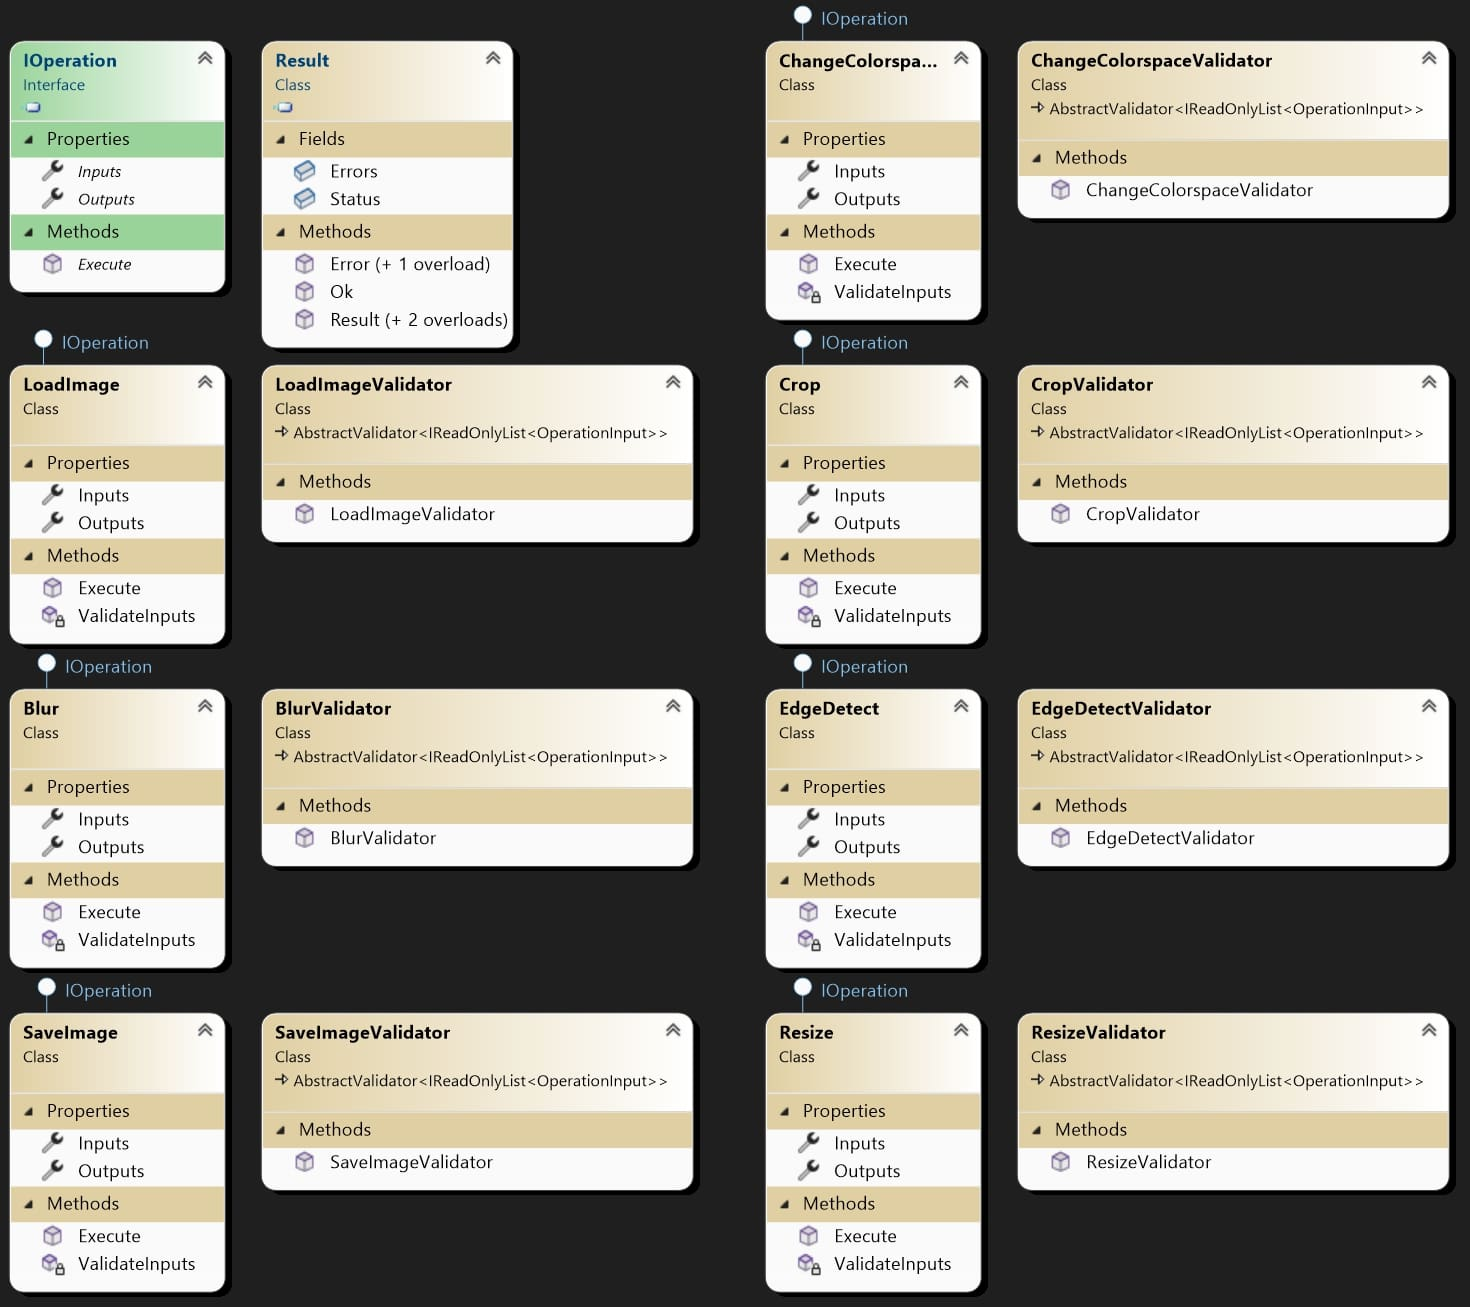
\includegraphics[height=5.3cm]{./imgs/operacje.jpg}
            \caption{Warstwa Model.}
    \end{figure}
\end{frame}

\begin{frame}{Architektura}
    \begin{figure}
            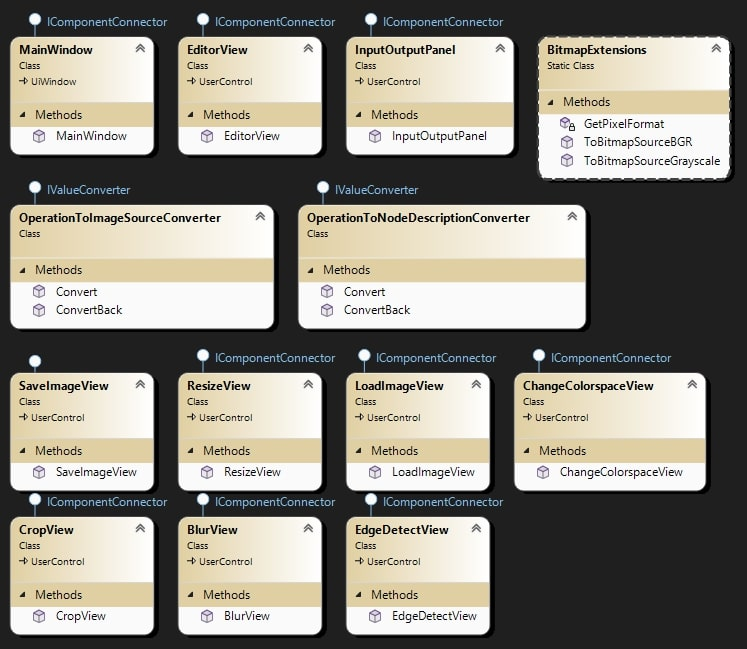
\includegraphics[height=6cm]{./imgs/widok.jpg}%
            \caption{Warstwa View.}
    \end{figure}
\end{frame}

\begin{frame}{Architektura}
    \begin{figure}
            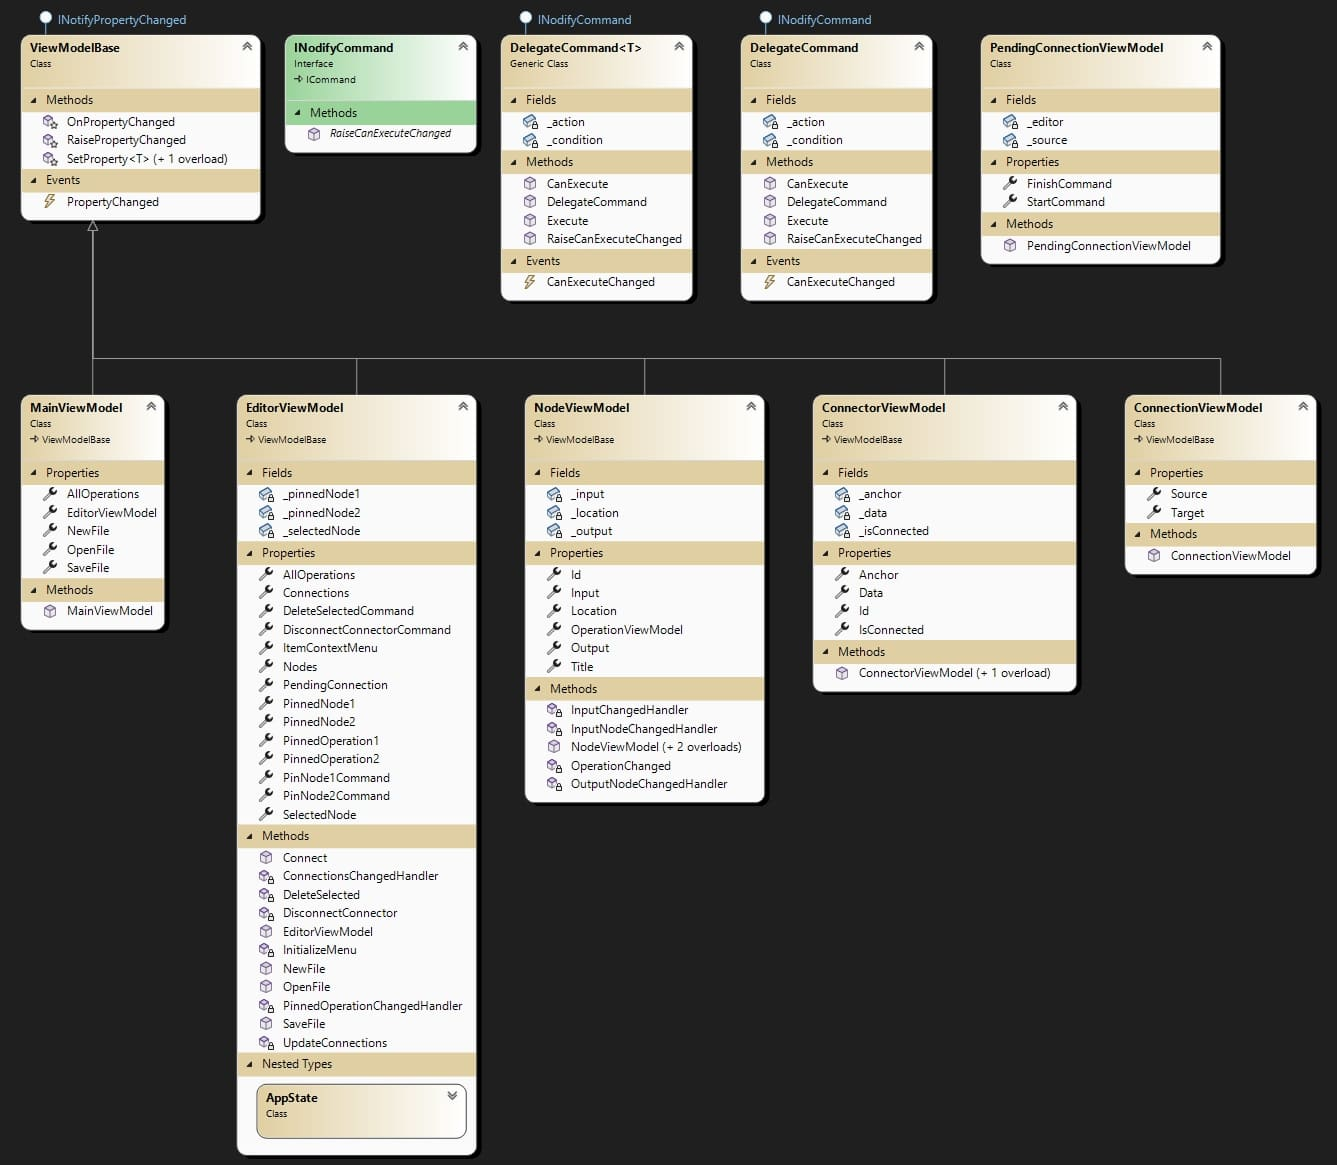
\includegraphics[height=5cm]{./imgs/vmedytor.jpg}%
            \hfil
            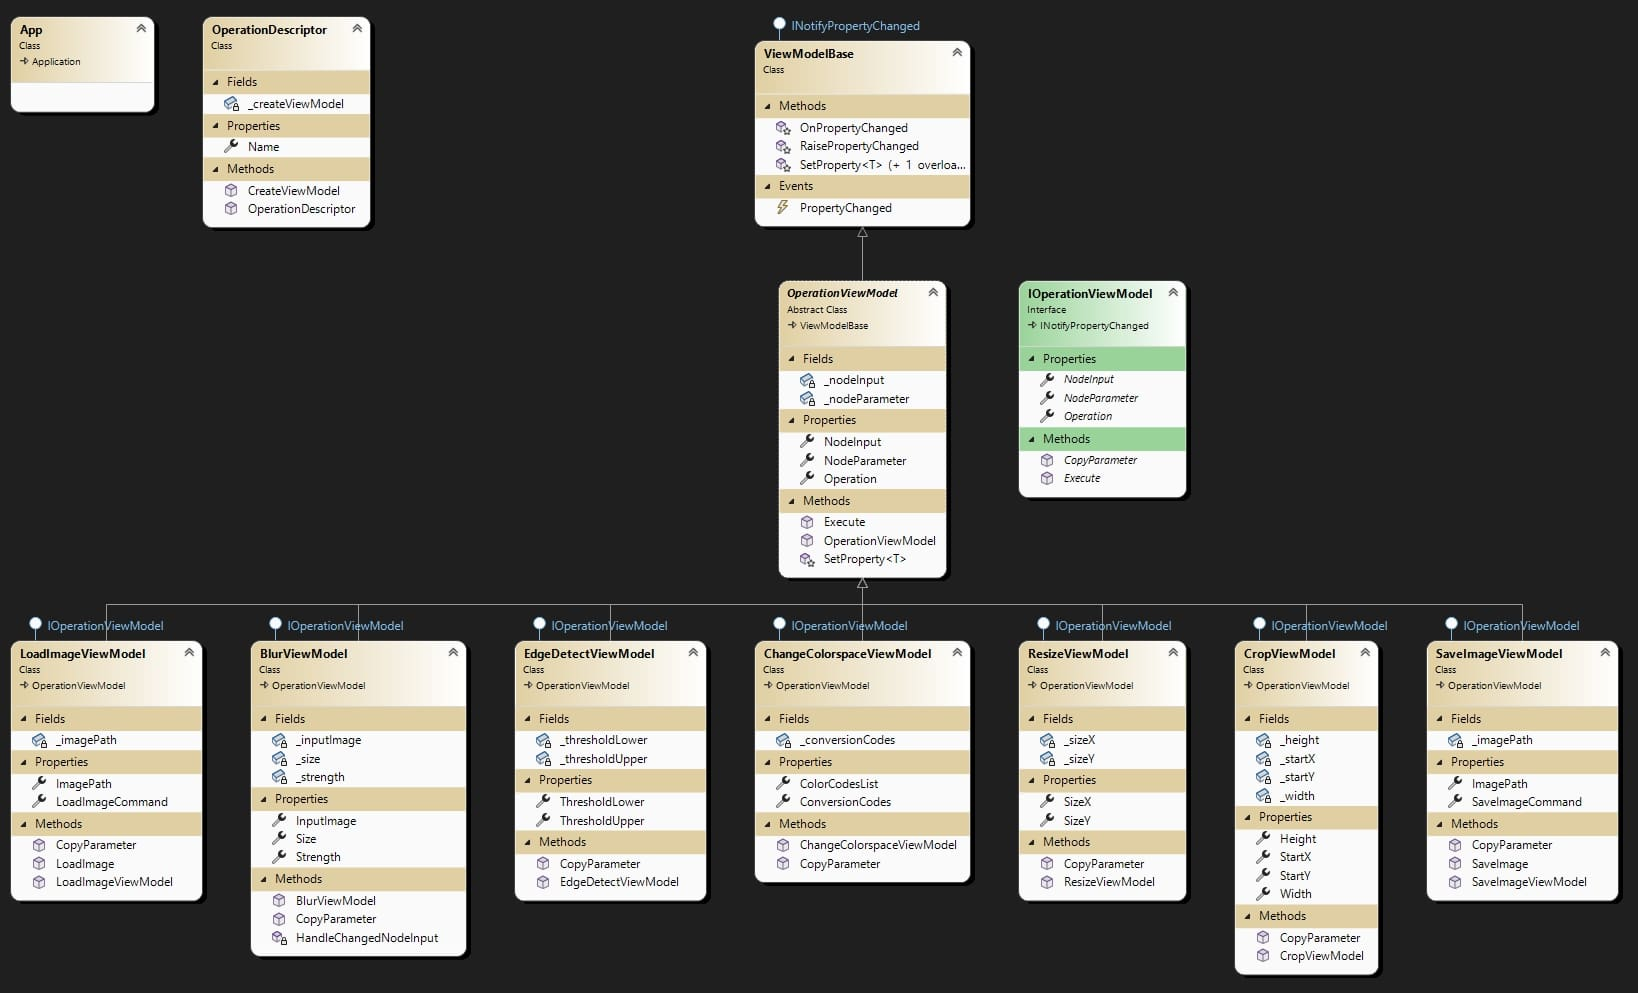
\includegraphics[height=5
            cm]{./imgs/vmoperacje.jpg}
            \caption{Warstwa ViewModelu.}
    \end{figure}
\end{frame}

\begin{frame}{Interfejs użytkowinika}
    \begin{figure}
        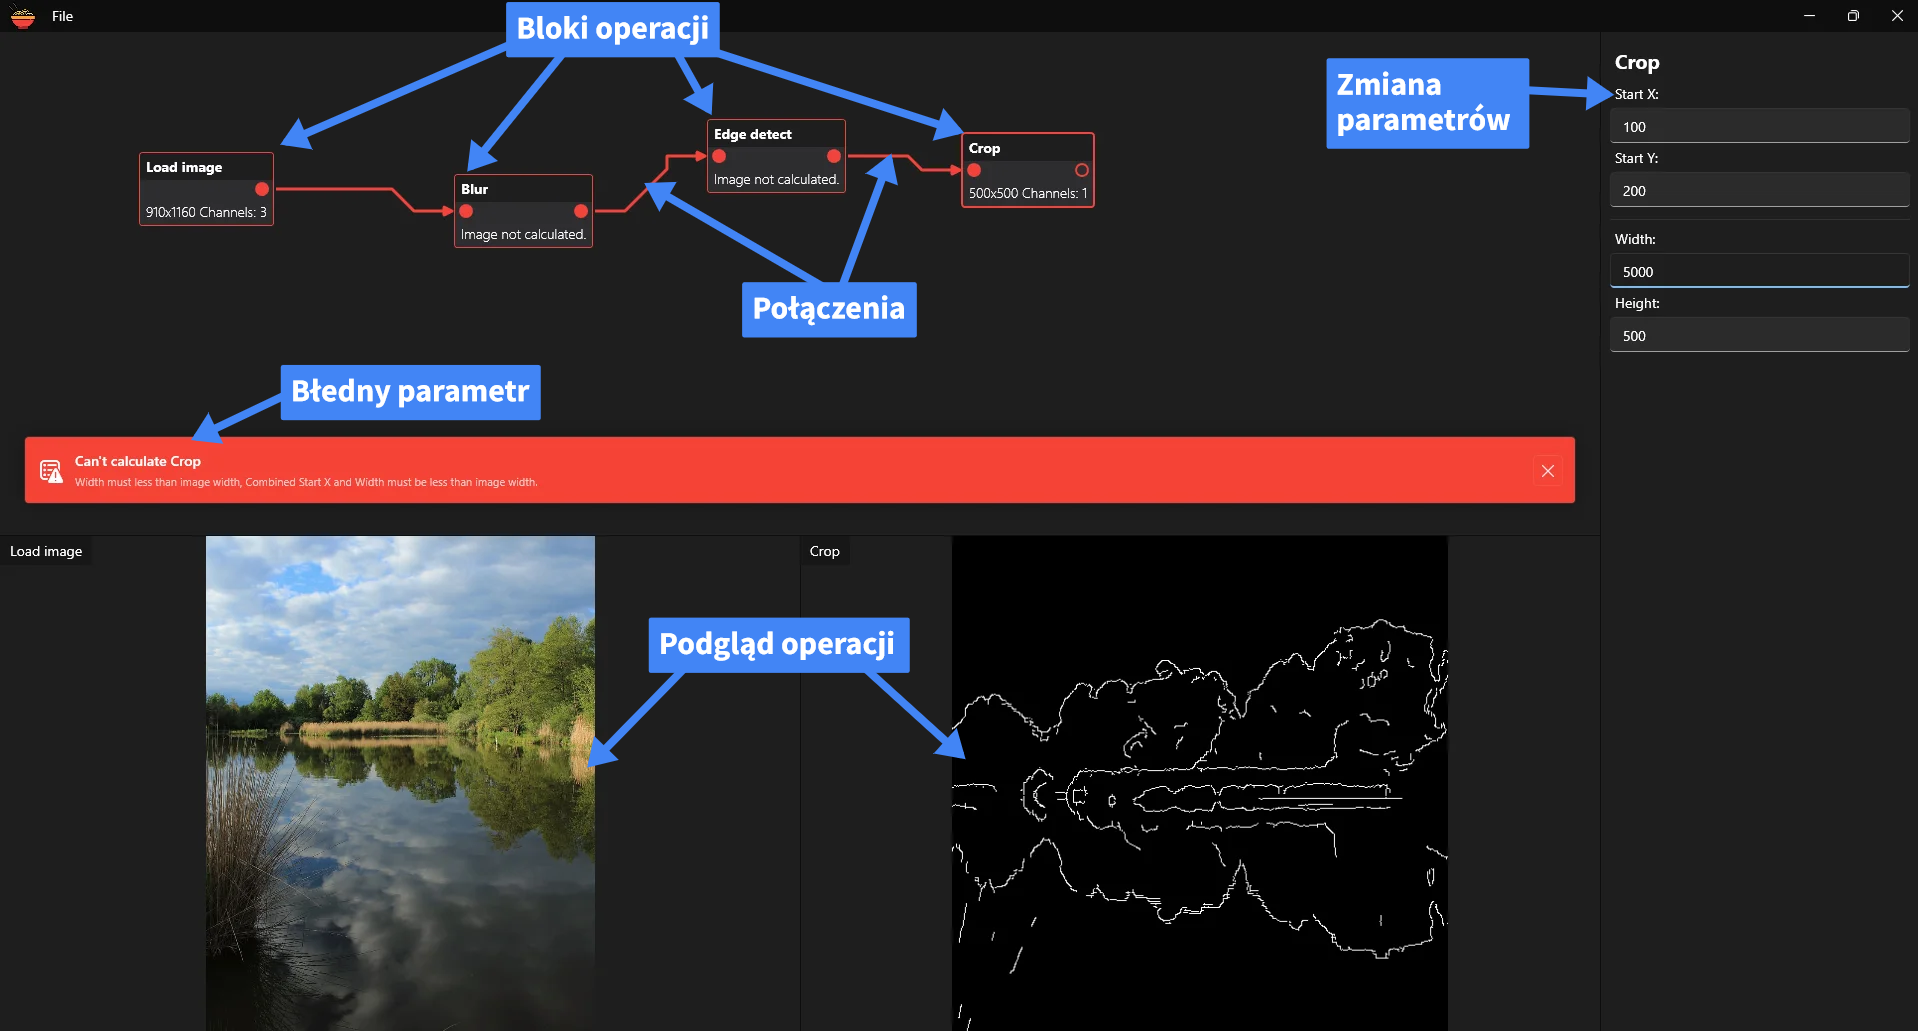
\includegraphics[height=6cm]{./imgs/interfejs.png}
        \caption{Wygląd przykładowej operacji.}
    \end{figure}
\end{frame}

\begin{frame}{Wykonanie}
    Prezentacja działania:
    \begin{itemize}
        \item \href{run:./imgs/long.mp4}{Działanie programu}
        \item \href{run:./imgs/opened.mp4}{Zapis i odczyt stanu}
        \item \href{run:./imgs/ui.mp4}{Interfejs}
    \end{itemize}
\end{frame}

\begin{frame}{Podsumowanie}
    Celem pracy było stworzenie aplikacji do przetwarzania obrazów z interfejsem graficznym.Interakcja użytkownika z programem odbywa się przez edytor węzłowy, a parametry odpowiadają tym używanym w bibliotece OpenCV. Wyniki obliczeń zostają wyświetlane natychmiastowo, a parametry które można wprowadzić są sprawdzane pod kątem poprawności. Cel został zrealizowany.
\end{frame}

\begin{frame}{Wnioski}
    \begin{itemize}
        \item Odpowiednia separacja logiki biznesowej i widoku ma znaczenie,
        \item użytkownik spodziewa się, że program zareaguje natychmiastowo na jego akcje,
        \item tworzenie narzędzi o takiej dowolności wymaga dużo walidacji,
        \item edytory węzłowe wymagają solidnej architektury.
    \end{itemize}
\end{frame}

\begin{frame}{Obszary do poprawy}
    \begin{columns}[t]
        \column{.5\textwidth}
        Pomysły z innych edytorów węzłowych:
        \begin{itemize}
            \item tworzenie i zapisywanie parametrów,
            \item łączenie kilku bloków w jeden przez użytkownika,
            \item grupowanie, układanie czy komentarzne,
            \item miniaturki z podglądem,
            \item eksportowanie pliku do edycji w zewnętrznych programach.
        \end{itemize}
        \column{.5\textwidth}
        Rozbudowa wsparcia biblioteki OpenCV:
        \begin{itemize}
            \item zwiększenie liczby metod dostępnych w aplikacji,
            \item wsparcie dla innych rodzajów danych jak wideo, chmury punktów itd.,
            \item użycie funkcji uczenia maszynowego lub sieci neuronowych,
            \item wybór metody gdy więcej niż jedna realizuje ten sam cel.
        \end{itemize}
    \end{columns}
\end{frame}

\end{document}